\documentclass[11pt,a4paper]{article}
\usepackage{amsmath,amssymb,amsthm}
\usepackage{graphicx}
\usepackage[margin=2.2cm]{geometry}
\usepackage{xcolor}
\usepackage{titlesec}
\usepackage{fancyhdr}
\usepackage{booktabs}
\usepackage{enumitem}
\usepackage{float}
\usepackage{hyperref}
\hypersetup{colorlinks=true,linkcolor=blue!70!black,urlcolor=blue!70!black}

\renewcommand{\topfraction}{0.9}
\renewcommand{\bottomfraction}{0.9}
\renewcommand{\textfraction}{0.07}
\renewcommand{\floatpagefraction}{0.7}
\setcounter{topnumber}{3}
\setcounter{bottomnumber}{3}
\setcounter{totalnumber}{5}

\definecolor{primary}{RGB}{0,51,102}
\definecolor{accent}{RGB}{204,102,0}

\titleformat{\section}{\Large\bfseries\color{primary}}{\thesection}{1em}{}
\titleformat{\subsection}{\large\bfseries\color{primary!80!black}}{\thesubsection}{1em}{}

\pagestyle{fancy}
\fancyhf{}
\fancyhead[L]{\small\color{primary}Essential Summary}
\fancyhead[R]{\small\color{primary}Li et al.\ (2013)}
\fancyfoot[C]{\thepage}
\renewcommand{\headrulewidth}{0.5pt}

\begin{document}

\begin{center}
{\LARGE\bfseries\color{primary}Essential Summary}\\[12pt]
{\large\bfseries A Generalized Harmonic Function Perturbation Method\\for Determining Limit Cycles and Homoclinic Orbits\\of Helmholtz--Duffing Oscillator}\\[8pt]
{\normalsize Zhenbo Li, Jiashi Tang, Ping Cai}\\[4pt]
{\small\itshape Journal of Sound and Vibration, Vol.\ 332, No.\ 21, 5508--5522 (2013)\quad DOI: 10.1016/j.jsv.2013.05.007}\\[6pt]
{\small\rule{0.7\textwidth}{0.5pt}}\\[4pt]
{\small\color{accent}This is an author-prepared essential summary, not the original paper.\\Please cite the published version.}
\end{center}

\vspace{0.5em}

\section{Background and Motivation}

The Helmholtz--Duffing oscillator, governed by $\ddot{x} + c_1 x + c_2 x^2 + c_3 x^3 = 0$, appears in ship dynamics, oscillations of the human eardrum, one-dimensional structural systems with initial curvature, and heavy symmetric gyroscopes. The asymmetric quadratic term $c_2 x^2$ breaks the symmetry present in classical Duffing oscillators, introducing qualitatively different dynamical behavior.

When perturbed by nonlinear damping, the oscillator
\begin{equation}
\ddot{x} + c_1 x + c_2 x^2 + c_3 x^3 = \varepsilon f(\mu, x, \dot{x})
\label{eq:model}
\end{equation}
exhibits limit cycles and homoclinic bifurcations. Unlike the Duffing oscillator (where $c_2=0$), the Helmholtz--Duffing oscillator requires a fundamentally different analytical treatment because its potential energy is asymmetric, and its exact solution cannot be expressed through standard elliptic functions alone.

This paper introduces the \textbf{generalized harmonic function perturbation (GHFP) method}---a novel perturbation framework that, for the first time, provides a unified treatment for both limit cycle determination and homoclinic orbit prediction in the damped Helmholtz--Duffing oscillator.

\section{Core Innovation: Quadratic Generalized Harmonic Function}

\subsection{Nonlinear Time Transformation}

The key innovation is the introduction of a nonlinear time transformation:
\begin{equation}
\frac{d\varphi}{dt} = \Phi(\varphi), \qquad \Phi(\varphi + \pi) = \Phi(\varphi)
\label{eq:NTT}
\end{equation}
that converts the time-domain equation into an angular-domain form over the symmetric interval $[0, \pi]$.

\subsection{Solution Construction}

The periodic solution is constructed as a \textbf{quadratic generalized harmonic function}:
\begin{equation}
\boxed{x(t) = a \cos^2\varphi(t) + b}
\label{eq:solution}
\end{equation}
where $a, b \in \mathbb{R}$. This representation differs fundamentally from prior approaches that used $x = a\cos\varphi + b$. The $\cos^2\varphi$ form automatically captures the asymmetry induced by the quadratic term $c_2 x^2$.

For homoclinic orbits, the solution takes the alternative form:
\begin{equation}
x(t) = a \sin^2\varphi(t) + b
\label{eq:homoclinic}
\end{equation}

\subsection{Determining $a$ and $b$}

Substituting Eq.~(\ref{eq:solution}) into the undamped oscillator and using Eq.~(\ref{eq:NTT}), the angular velocity $\Phi(\varphi)$ is obtained as:
\begin{equation}
\Phi(\varphi) = \sqrt{\frac{2[V(a+b) - V(a\cos^2\varphi + b)]}{(x'(\varphi))^2}}
\label{eq:Phi}
\end{equation}
where $V(x) = \int_0^x g(u)du$ and $g(x) = c_1 x + c_2 x^2 + c_3 x^3$.

The constants $a$ and $b$ are determined by:
\begin{equation}
\int_{a+b}^b g(u)du = 0
\label{eq:constants}
\end{equation}
and $a+b = x(0)$ (the initial condition). For homoclinic orbits, the saddle point $h$ satisfies $g(h)=0$, and the initial condition $c$ is determined by $\int_h^c g(x)dx = 0$.

\section{The GHFP Perturbation Procedure}

\subsection{Perturbation Expansion}

When $\varepsilon \neq 0$, the solution parameters are expanded in powers of $\varepsilon$:
\begin{equation}
a = a_0 + \varepsilon a_1 + \cdots, \qquad \Phi = \Phi_0 + \varepsilon \Phi_1 + \cdots
\label{eq:expansion}
\end{equation}

Substituting into Eq.~(\ref{eq:model}) and equating coefficients of like powers of $\varepsilon$ yields a hierarchy of equations:
\begin{align}
\varepsilon^0&: \quad \frac{d}{d\varphi}(\Phi_0^2 x_0') + g(x_0) = 0 \\
\varepsilon^1&: \quad \frac{d}{d\varphi}(\Phi_0\Phi_1 x_0' + \Phi_0^2 x_1') + g'(x_0)x_1 = f(\mu, x_0, \Phi_0 x_0')
\end{align}

\subsection{Key Assumption}

The critical assumption that simplifies the perturbation procedure: \textbf{the $n$th-order approximate solution $x_n$ has the same functional form as the generating solution}:
\begin{equation}
x_n = a_n \cos^2\varphi \quad (\text{or } x_n = a_n \sin^2\varphi \text{ for homoclinic orbits})
\label{eq:assumption}
\end{equation}
This eliminates the cumbersome integration required in classical perturbation methods.

\subsection{Central Result: Bifurcation Parameter Prediction}

The first-order consistency condition (obtained by integrating the $\varepsilon^1$ equation over $[0, \pi]$) yields:
\begin{equation}
\boxed{\mu = -\frac{\int_0^\pi \Phi_0 f_0(\mu, x_0, \Phi_0 x_0') x_0' d\varphi}{\int_0^\pi \Phi_0 \frac{\partial f_0}{\partial \mu} x_0' d\varphi}}
\label{eq:bifurcation}
\end{equation}
This formula directly gives the critical value of the control parameter $\mu_c$ at which homoclinic bifurcation occurs---previously obtainable only through numerical shooting methods.

\section{Key Results}

\subsection{Example 1: $c_1=1$, $c_2=0.5$, $c_3=1$}

Consider the damped Helmholtz--Duffing oscillator:
\begin{equation}
\ddot{x} + x + 0.5x^2 + x^3 = \varepsilon(\mu + \mu_1 x + \mu_2 x^2)\dot{x}
\label{eq:ex1}
\end{equation}

\begin{figure}[htbp]
\centering
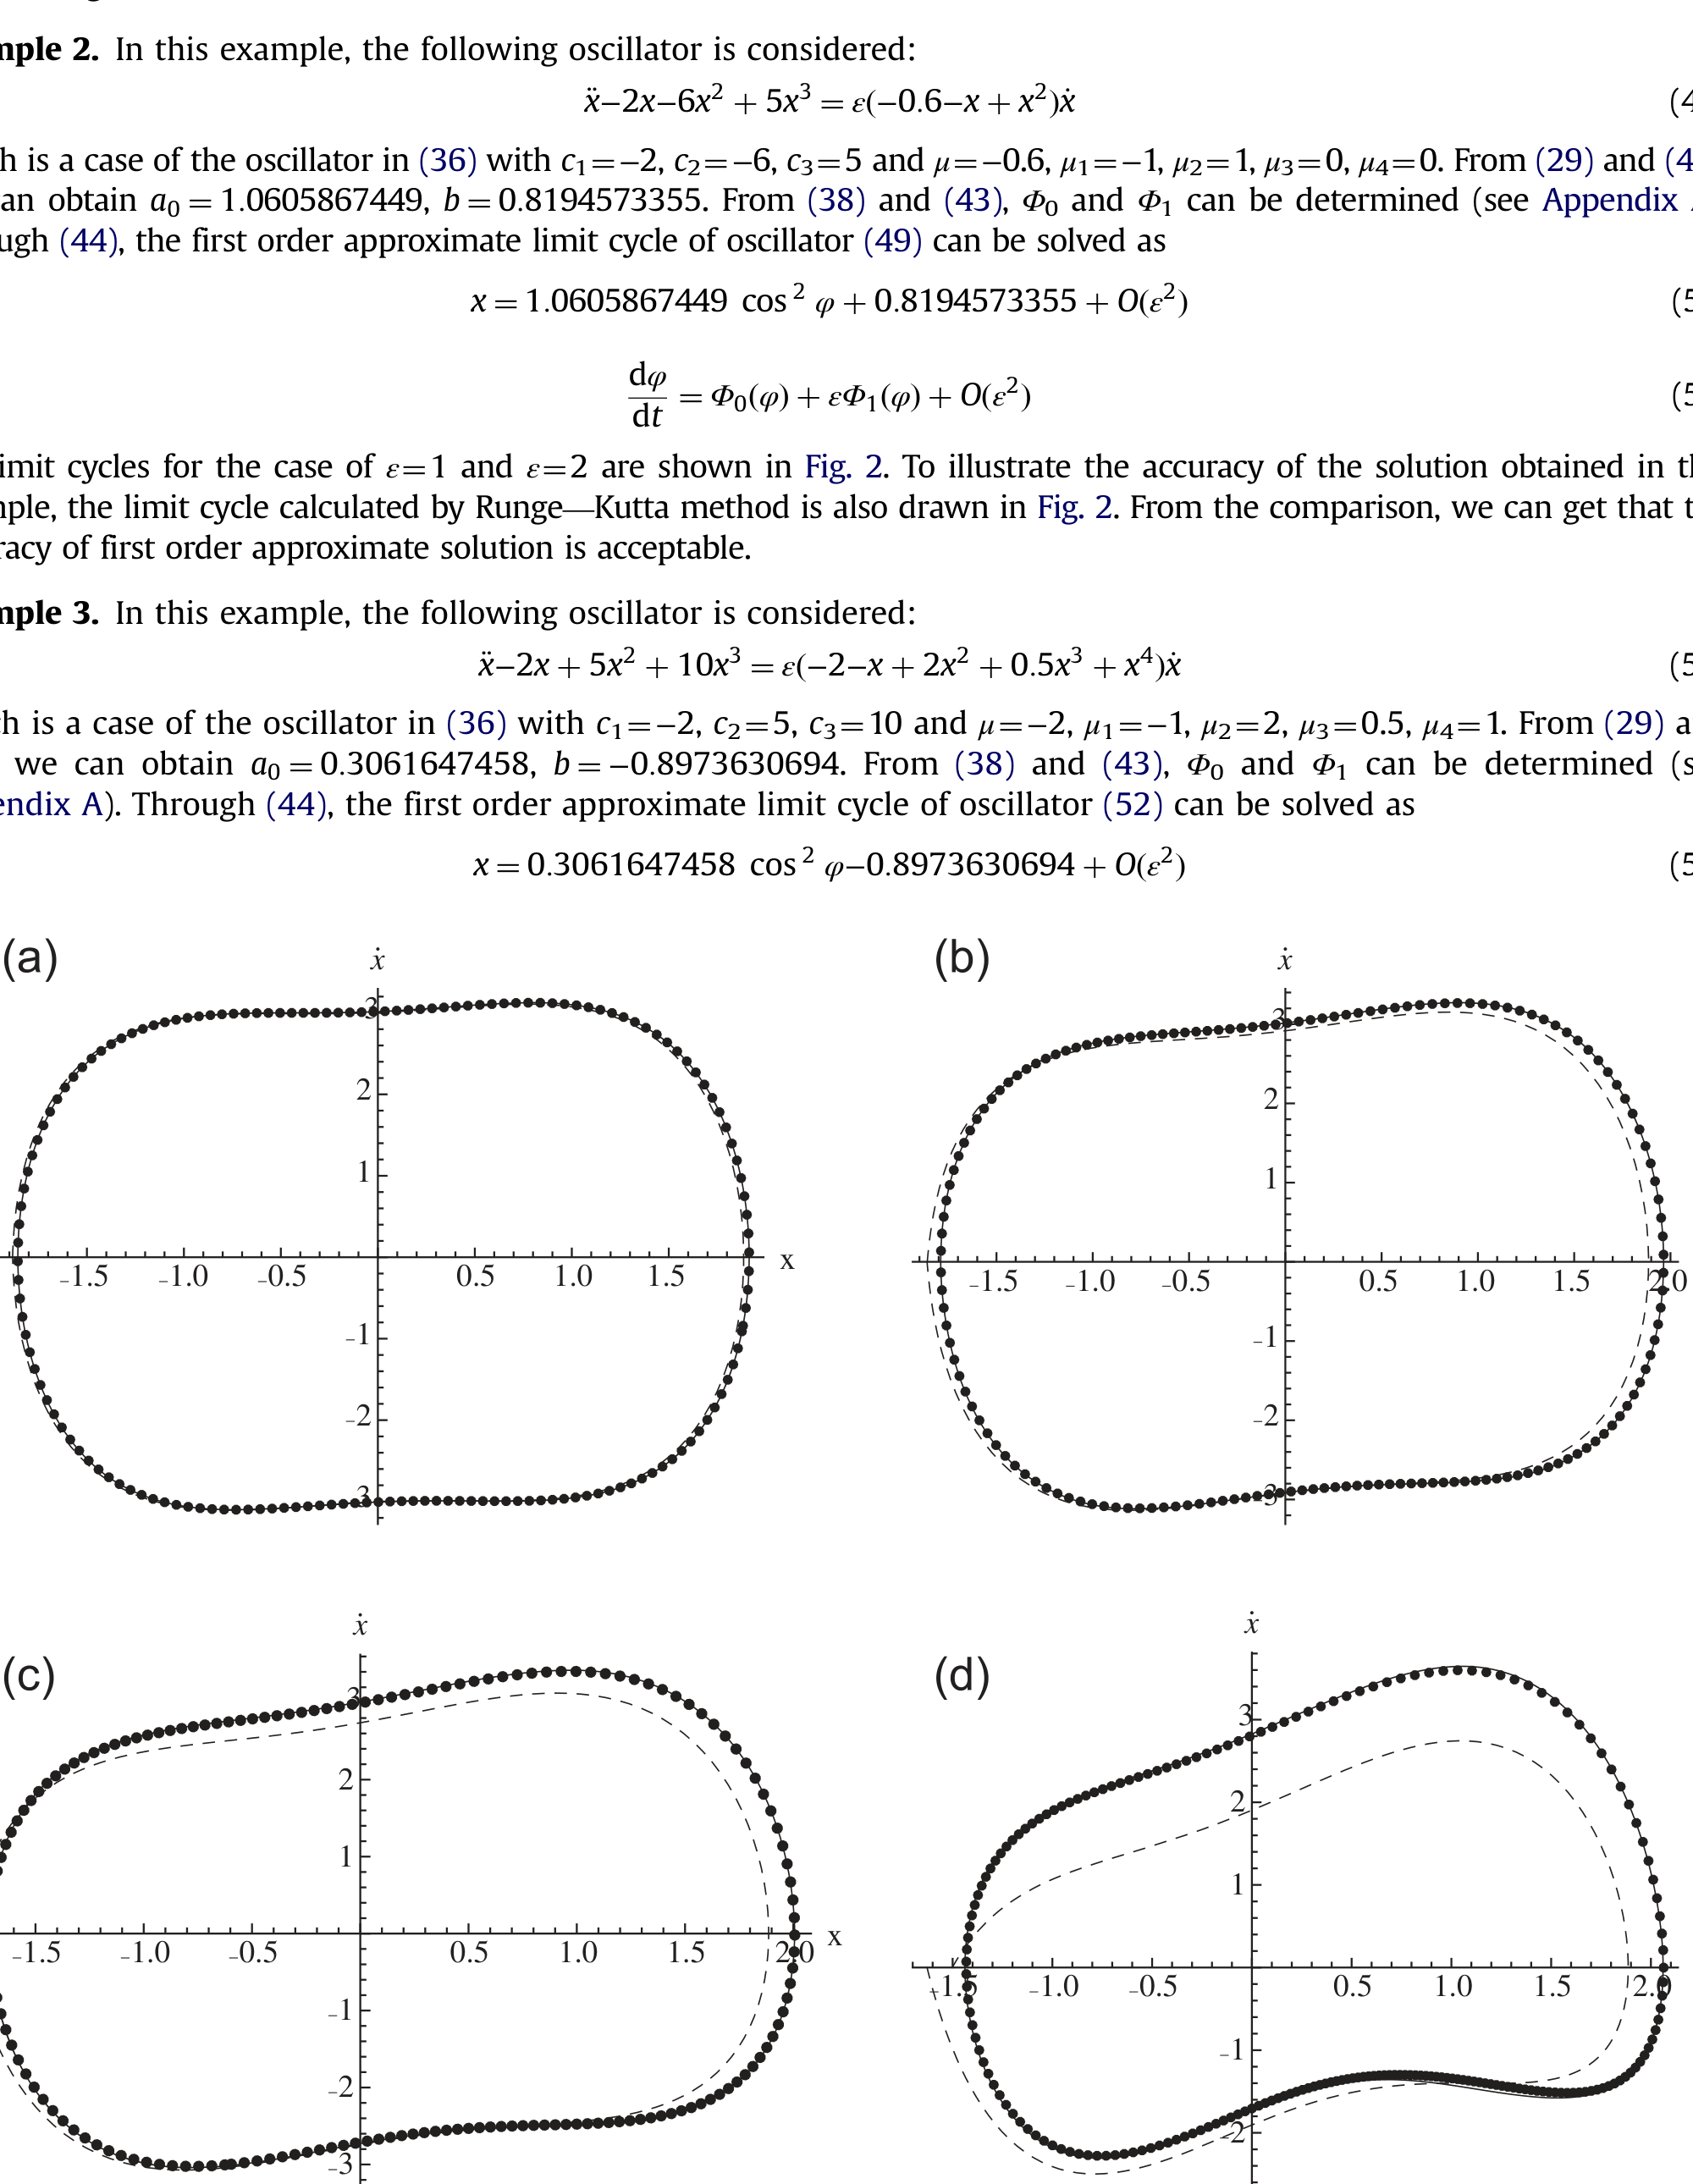
\includegraphics[width=\textwidth,height=0.42\textheight,keepaspectratio]{p5-fig1-limitcycle.png}
\caption{\textbf{Figure 1.} (Original Fig.\ 1) Limit cycles of oscillator (\ref{eq:ex1}) for $\varepsilon=0.1, 0.3, 0.5, 1$. Solid lines: Runge--Kutta method. Dotted lines: GHFP method. Excellent agreement at all perturbation levels demonstrates the method's accuracy.}
\end{figure}

\subsection{Example 2: $c_1=1$, $c_2=-1$, $c_3=2$---Homoclinic Orbits}

\begin{equation}
\ddot{x} + x - x^2 + 2x^3 = \varepsilon(\mu + \mu_2 x^2)\dot{x}
\label{eq:ex2}
\end{equation}

This oscillator possesses a saddle point at $x=0$ and two additional equilibrium points, enabling homoclinic bifurcation. The critical parameter values predicted by the GHFP method are in close agreement with numerical results.

\begin{figure}[htbp]
\centering
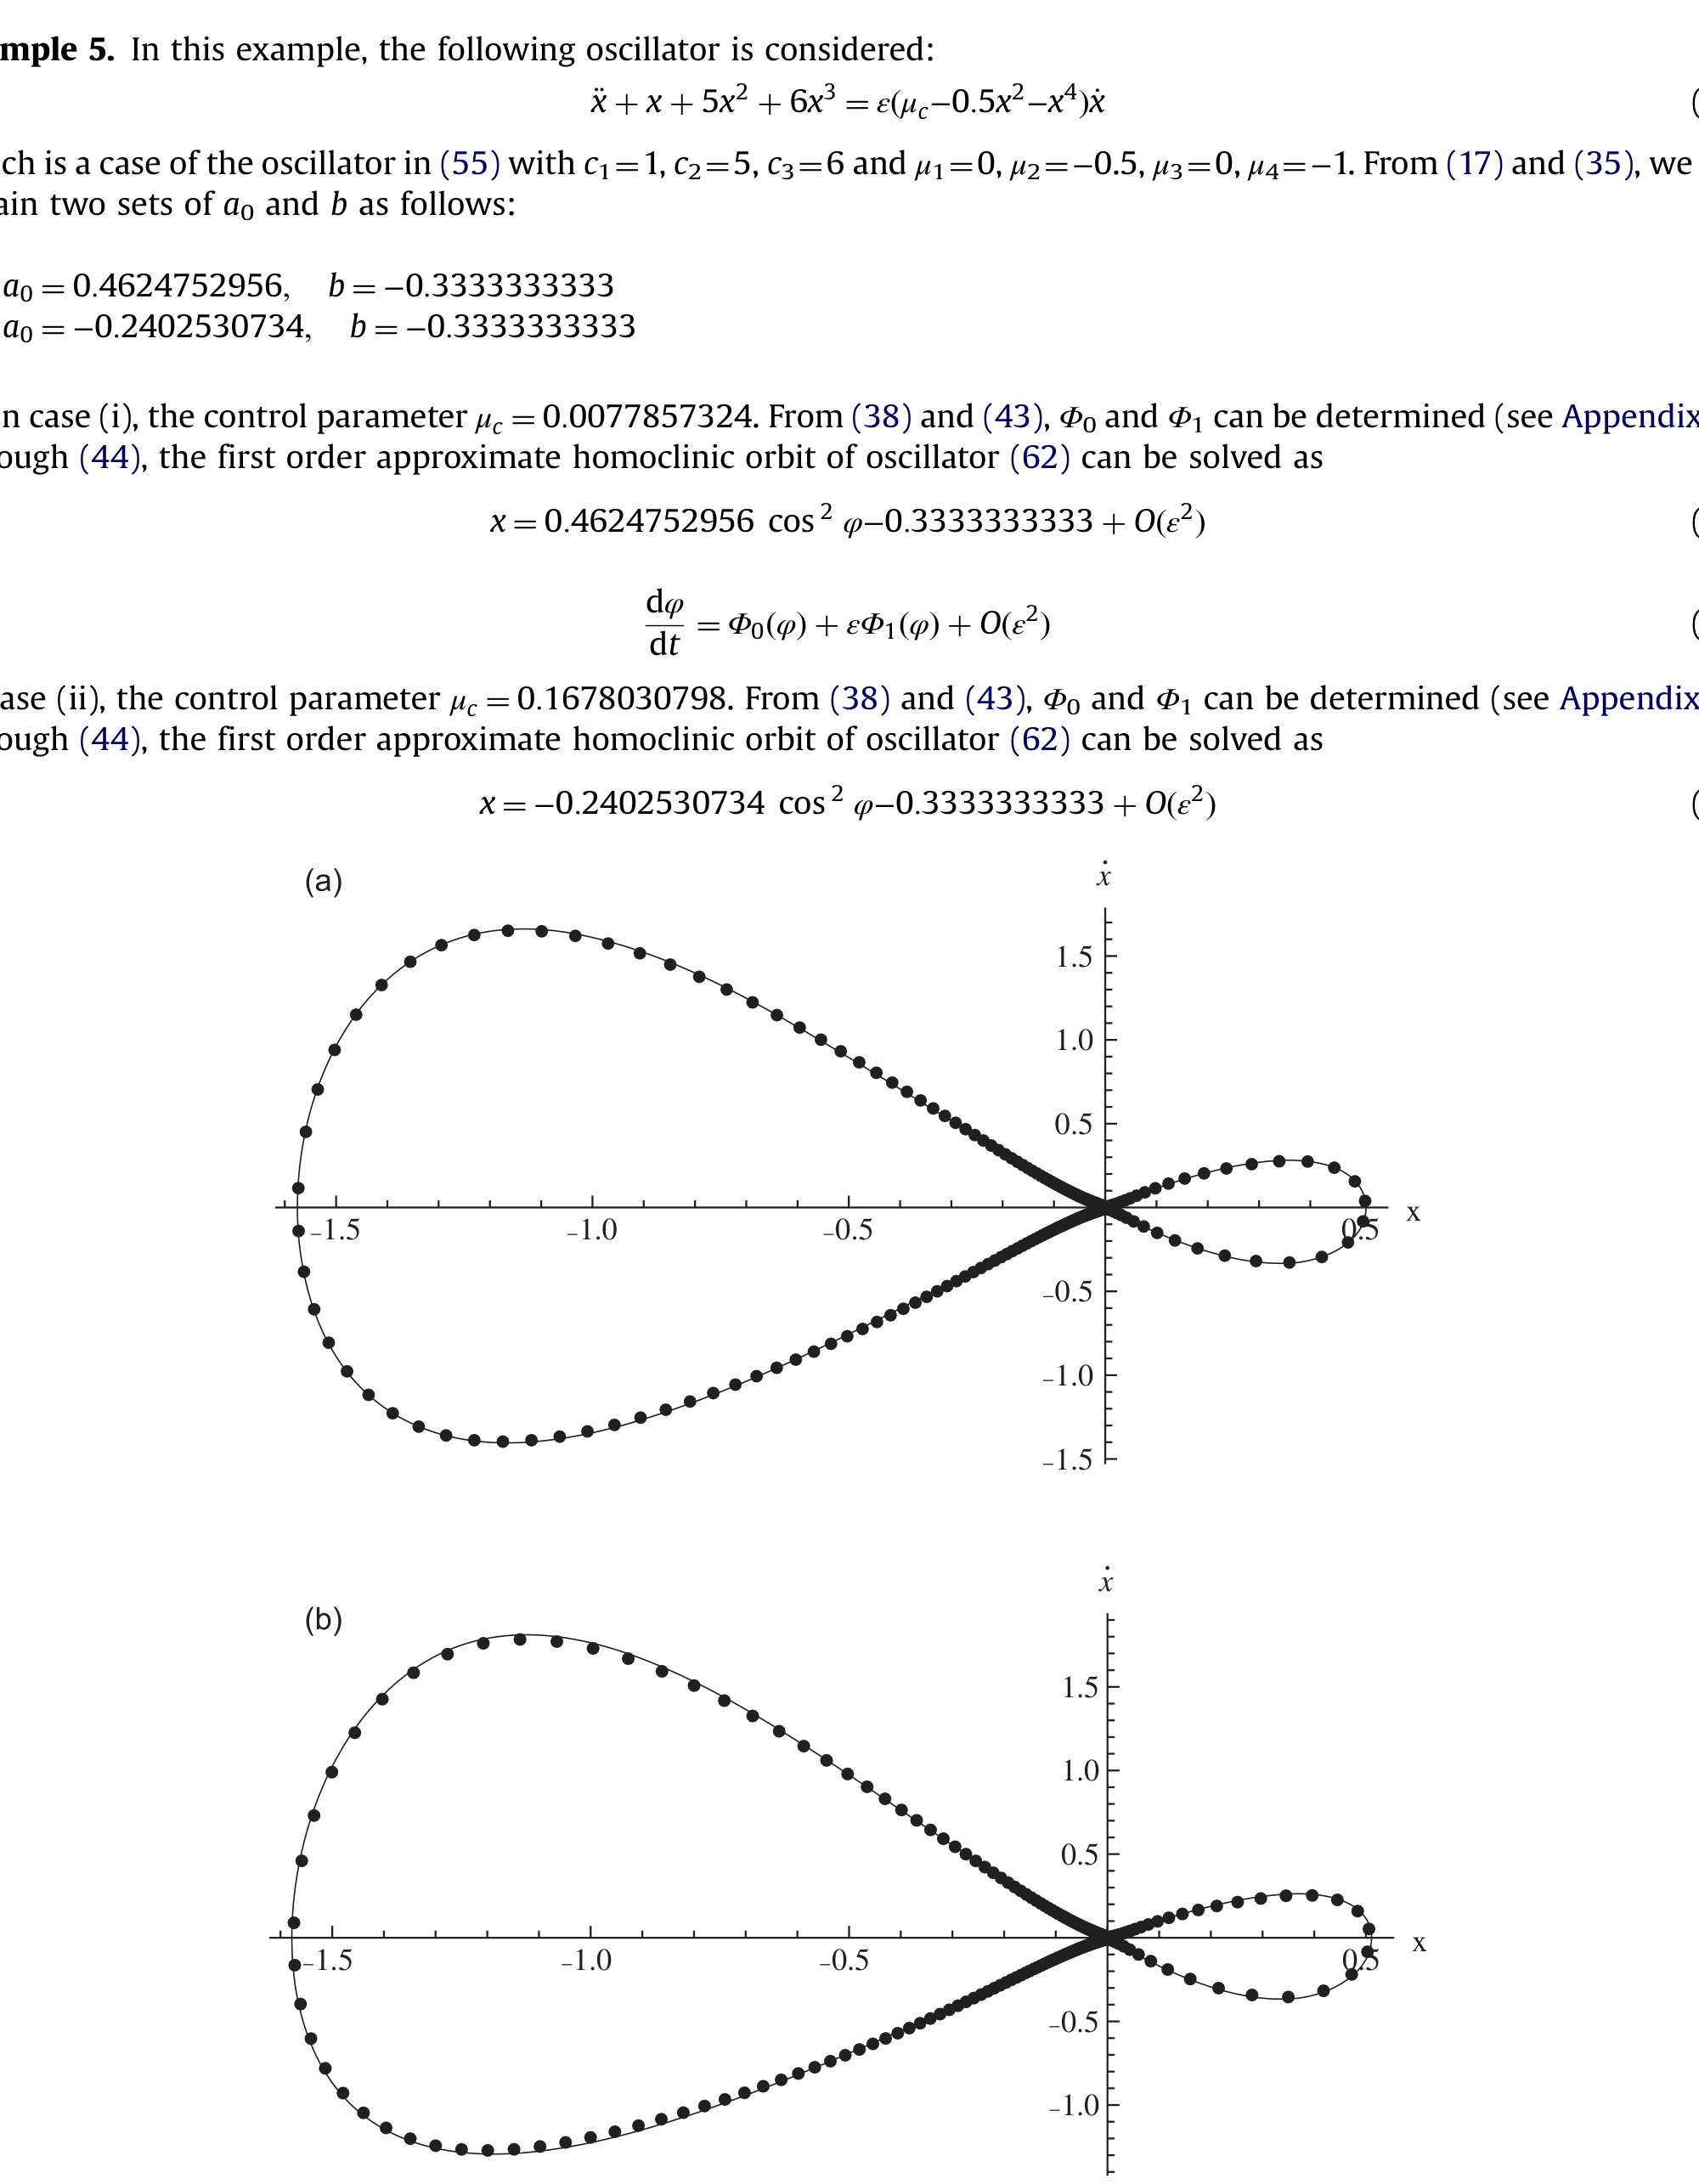
\includegraphics[width=0.85\textwidth,height=0.40\textheight,keepaspectratio]{p5-fig5-homoclinic.png}
\caption{\textbf{Figure 2.} (Original Fig.\ 5) Homoclinic orbits of oscillator (\ref{eq:ex2}) for $\varepsilon=1, 2$. Solid lines: Runge--Kutta. Dotted lines: GHFP method. The method accurately captures homoclinic orbit geometry even at $\varepsilon=2$.}
\end{figure}

\section{Significance and Impact}

\begin{enumerate}[leftmargin=2em]
\item \textbf{Foundation of the GHFP family:} This paper establishes the quadratic generalized harmonic function framework---the foundation upon which all subsequent GHFP and MGHFP methods are built. The insight that $x = a\cos^2\varphi + b$ (rather than $a\cos\varphi + b$) is the correct basis function for asymmetric oscillators proved essential.

\item \textbf{First analytical homoclinic bifurcation prediction:} Before this work, predicting the critical parameter for homoclinic bifurcation in strongly nonlinear oscillators required numerical shooting. The GHFP method provides the first analytical formula.

\item \textbf{Unified treatment of limit cycles and global bifurcations:} The same framework handles both local (limit cycle) and global (homoclinic/heteroclinic) dynamical phenomena, eliminating the need for separate analytical approaches.
\end{enumerate}

\section{Limitations}

\begin{itemize}[leftmargin=2em]
\item The method is limited to first-order perturbation accuracy; higher-order extensions would improve precision for larger $\varepsilon$.
\item The approach assumes the nonlinear damping is small ($\varepsilon \ll 1$); strongly damped systems require alternative treatments.
\item Only single-degree-of-freedom oscillators are considered; multi-degree-of-freedom extensions remain an open challenge.
\end{itemize}

\vfill
\begin{center}
\small\rule{0.5\textwidth}{0.3pt}\\[4pt]
\small\color{primary} Author: Zhenbo Li (lizhenbo@usc.edu.cn)\\
\small University of South China, School of Mathematics and Physics\\
\small Hunan Key Laboratory of Mathematical Modeling and Scientific Computing
\end{center}

\end{document}
